\documentclass[tikz]{standalone}
\usepackage{pgfplots}
\pgfplotsset{compat=1.15}
\usepackage{mathrsfs}
\usetikzlibrary{arrows,calc}
\usepackage{tkz-euclide}
\pagestyle{empty}
\usepackage{fp}

\definecolor{AngleClr}{rgb}{0,0.39215686274509803,0}
\definecolor{ShapeClr}{rgb}{0.6,0.2,0}

\begin{document}

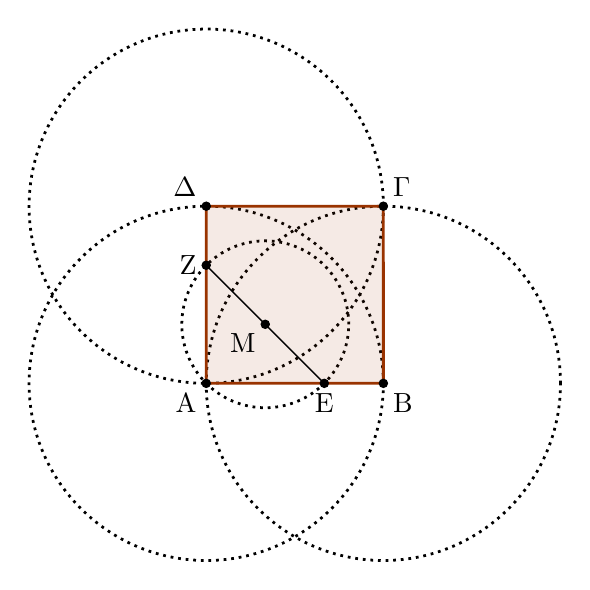
\begin{tikzpicture}[scale=.75]
\tkzSetUpLine[line width=1pt,color=black]
\tkzSetUpPoint[fill=black]

\tkzDefPoints{0/0/A,3/0/B,1/1/M}

% Step 2.
\tkzDrawCircle[line width=1.0pt, color=black,dashed,dash pattern=on 1pt off 1.75pt](M,A)

% Step 3.
\tkzInterLC(A,B)(M,A) \tkzGetPoints{ZZ}{E}

% Step 4.
\tkzInterLC(M,E)(M,A) \tkzGetPoints{Z}{ZZ}

% Step 5. 
\tkzDrawCircle[line width=1.0pt, color=black,dashed,dash pattern=on 1pt off 1.75pt](A,B)
\tkzInterLC(A,Z)(A,B) \tkzGetPoints{ZZ}{D}

% Step 6
\tkzDrawCircle[line width=1.0pt, color=black,dashed,dash pattern=on 1pt off 1.75pt](B,A)
\tkzDrawCircle[line width=1.0pt, color=black,dashed,dash pattern=on 1pt off 1.75pt](D,A)
\tkzInterCC(B,A)(D,A) \tkzGetPoints{ZZ}{C}

\tkzFillPolygon[fill=ShapeClr,fill opacity=0.1,inner sep=1cm](A,B,C,D)

\tkzDrawSegment[line width=0.5pt,color=black](A,B)

\tkzDrawSegment[line width=0.5pt,color=black](M,E)
\tkzDrawSegment[line width=0.5pt,color=black](M,Z)

\tkzDrawPolygon[color=ShapeClr](A,B,C,D)

\tkzDrawPoints[size=3](A,B,M,E,Z,D,C)

\tkzLabelPoint[below left](A){$\rm A$}
\tkzLabelPoint[below right](B){$\rm B$}
\tkzLabelPoint[below left](M){$\rm M$}
\tkzLabelPoint[below](E){$\rm E$}
\tkzLabelPoint[left](Z){$\rm Z$}
\tkzLabelPoint[above left](D){$\rm \Delta$}
\tkzLabelPoint[above right](C){$\rm \Gamma$}

\end{tikzpicture}

\end{document}
